\section{Газовые законы}
%TODO Время удара футбольного мяча

\begin{ex} 
(2001) Какой максимальной температуры достигнет 1 моль идеального газа в процессе, изображенном на рисунке? 
\begin{center}
\includestandalone{Pictures/082001GasLawsProcess}
\end{center}
\begin{sol}
Из уравнения Менделеева-Клапейрона $$T = \frac{pV}{\nu R}.$$
Из рисунка видно, что зависимость между давлением $p$ и объёмом $V$ линейная $$p(V)=KV+p_{0},$$ где $K = \tan \alpha = - \frac{p_{0}}{V_{0}}.$
Подставим $p(V)$ в выражение для $T$: 	$$T = \frac{(KV+p_{0})V}{\nu R}.$$
Воспользуемся стандартным методом из математического анализа для поиска максимальной температуры $$\frac{dT}{dV} = 0,$$ $$\frac{1}{\nu R}(2VK+p_{0})=0,$$ $$2VK+p_{0}=0,$$ $$2\frac{p_{0}}{V_{0}}V=p_{0},$$ $$V=\frac{V_{0}}{2}.$$
$$T_{max} = T\left(\frac{V_{0}}{2}\right)=\frac{p_{0}V_{0}}{4\nu R}.$$
\end{sol}
\begin{ans}
$T_{\max}=p_0V_0/(4R)$
\end{ans}
\end{ex}

\begin{ex}
Найдите максимальную температуру идеального газа в процессе, протекающем по закону $P=P_0~-~\alpha~V^2$, где $P_0$ и $\alpha$ -- положительные постоянные, $V$ -- объем одного моля.
\begin{ans}
$T_{\max} = \sqrt{p_0/3\alpha}$
\end{ans}
\end{ex}

\begin{ex}
(2010) Посередине откаченной и запаянной с обоих концов горизонтально расположенной трубки длины $L$ находится столбик ртути длины $h$. 
Если трубку поставить вертикально, столбик ртути сместится на расстояние $x$. Какое первоначальное давление в трубке? Плотность ртути $\rho$.
\begin{sol}
Так как в горизонтальном положении столбик ртути посередине, то температура газа в полостях по обе стороны от столбика одинаковая. Из уравнения Менделеева-Клапейрона: $$p_{0}V_{0}=\nu RT_{0},$$ где $p_{0}$ -- искомое давление, $V_{0} = \dfrac{(L-h)S}{2}$ -- объём каждого из столбов газа,
$$\Rightarrow p_{0} = \dfrac{\nu RT_{0}}{V_{0}}.$$
Силы, действующие на столбик в вертикальном положении: $$p_{1}S=p_{2}S+F,$$ где $p_{1}$ -- давление нижнего столба, $p_{2}$ -- давление верхнего столба, $F$ -- сила тяжести, действующая на столбик с ртутью, $S$ -- площадь поперечного сечения трубки.
Для идеального газа справедливо: $$p_{1}V_{1} = \nu RT_{0},$$ $$p_{2}V_{2}=\nu RT_{0}.$$ Откуда $$p_{1} = \dfrac{\nu RT_{0}}{V_{1}},$$ где $V_{1} = \left(\dfrac{L-h}{2}-x\right)S$ и $$p_{2} = \dfrac{\nu RT_{0}}{V_{2}},$$ где $V_{2} = \left(\dfrac{L-h}{2}+x\right)S$.
Используем полученные выражения и переписываем уравнение для сил: $$F = S(p_{1} - p_{2}) = S \nu RT_{0}\left(\dfrac{1}{V_{1}}-\dfrac{1}{V_{2}}\right)=\dfrac{4x}{(L-h)^2-4x^2}2\nu RT_{0}.$$
$$p_{0} = \dfrac{1}{2V_{0}} \dfrac{(L-h)^2-4x^2}{4x}F= \dfrac{2}{2(L-h)S} \dfrac{(L-h)^2-4x^2}{4x}\rho hSg = \rho gh\dfrac{(L-h)^2-4x^2}{4x(L-h)}.$$
\end{sol}
\begin{ans}
$p_0 = \rho g h \left( (L-h)^2 - 4x^2 \right)/ (4x(L-h))$
\end{ans}
\end{ex}

\begin{ex}
(2013) В баллон, вместимостью $V$, при давлении $p$ нагнетают воздух. За какое время $t$ он будет накачан до давления $p_n$, если компрессор за время $\tau$ засасывает объем $V_0$ атмосферного воздуха? 
Температуру считать неизменной, а атмосферное давление равным $p_0$. Как изменится ответ, если воздух откачивать из баллона?
\begin{ans}
$t_1 = \tau V(p_n-p)/(p_0V_0)$, $t_2 = \tau \log p/p_n /\log (1+V_0/V)$
\end{ans}
\end{ex}

\begin{ex}
\hspace{0pt} \\
\begin{minipage}{.65\textwidth}
(2012) На поверхности жидкости плотностью $\rho$ плавает тонкостенный цилиндрический стакан высотой $h$, наполовину погруженный в жидкость. 
На какую глубину $h_1$ погрузится стакан в жидкость, если его осторожно положить на поверхность жидкости вверх дном? 
На какую глубину $h_2$ нужно утопить перевернутый вверх дном стакан, чтобы он вместе с заключенным в нем воздухом пошел ко дну? Давление атмосферы $p_0$.
\end{minipage}
\begin{minipage}{.35\textwidth}
\centering
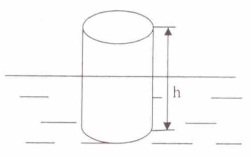
\includegraphics[width = 0.9 \textwidth]{082012GasLawsGlass.jpg}
\end{minipage}
\begin{ans}
$h_1 = h \frac{2p_0+3\rho gh}{2(2p_0 + \rho gh)}$, $h_2 = h/2 + p_0/\rho g$
\end{ans}
\end{ex}

%Бутиков
\begin{ex}
\hspace{0pt} \\
\begin{minipage}{.65\textwidth}
В вертикальном закрытом сосуде имеется поршень, который может перемещаться без трения. 
По обе стороны от поршня находятся одинаковые массы одного и того же газа. 
При температуре $T$ объем верхней части в $n$ раз больше, чем объем нижней. 
Каким будет соотношение этих объемов, если повысить температуру до значения $T_2$?
\end{minipage}
\begin{minipage}{.35\textwidth}
\centering
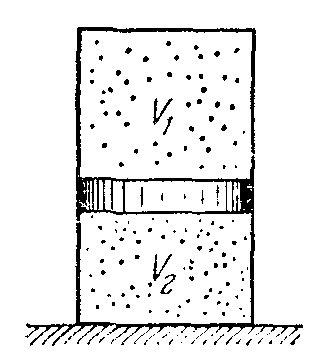
\includegraphics[width = 0.75 \textwidth]{0805GasLawsPiston.jpg}
\end{minipage}
\begin{sol}
\hspace{0pt} \\
\begin{minipage}{.5\textwidth}
При температуре $T$ запишем в виде системы уравнение статики для поршня, уравнения идеального газа и начальное соотношение объёмов, введём величину, представляющую собой сумму этих объёмов:
		\begin{equation}
		\begin{cases}
		mg + p_{1}S = p_{2}S\\
		p_{1}V_{1}=\nu RT\\
		p_{2}V_{2}=\nu RT\\
		\dfrac{V_{1}}{V_{2}}=n\\
		V_{1}+V_{2}=V,
		\end{cases}
		\end{equation}
где $p_{1}, p_{2}$ -- давление газа над и под поршнем соответственно.
Из полученной системы: $$V=V_{2}(n+1),$$ $$p_{2}=p_{1}n.$$ Тогда $mg=Sp_{1}(n-1)$ $$\Rightarrow p_{1}=\dfrac{mg}{S(n-1)} \Rightarrow p_{2}=\dfrac{nmg}{S(n-1)}.$$
С учётом полученных выкладок: $$V_{2} = \dfrac{\nu RT}{p_{2}}=\dfrac{S(n-1)}{nmg}\nu RT.$$
Тогда $V=\dfrac{S(n^2-1)}{nmg}\nu RT.$
\end{minipage}
\begin{minipage}{.5\textwidth}
Запишем аналогичную систему уравнений при температуре $T_{2}$:
\begin{equation}
\begin{cases}
mg + p_{1}^{'}S = p_{2}^{'}S\\
p_{1}^{'}V_{1}^{'}=\nu RT\\
p_{2}^{'}V_{2}^{'}=\nu RT\\
\dfrac{V_{1}^{'}}{V_{2}^{'}}=x\\
V_{1}^{'}+V_{2}^{'}=V.
\end{cases}
\end{equation}
Откуда $V=V_{2}^{'}(x+1)$ $$\Rightarrow x=\dfrac{V}{V_{2}^{'}}-1.$$
Аналогично $V_{2}$ получаем: $$V_{2}^{'}=\dfrac{\nu RT_{2}}{p_{2}^{'}}=\dfrac{S(x-1)}{xmg}\nu RT_{2}.$$
Тогда $$x=\dfrac{S(n^2-1)\nu RT}{nmg}\dfrac{xmg}{S(x-1)\nu RT_{2}}-1$$ $$\Rightarrow \dfrac{x^2-1}{x}=\dfrac{(n^2-1)T}{nT_{2}}=B.$$
Из решения $x^2-Bx-1=0$ получаем: $$x=\dfrac{(n^2-1)T}{2nT_{2}}+\sqrt{\left(\dfrac{(n^2-1)T}{2nT_{2}}\right)^2+1}.$$
\end{minipage}
\end{sol}
\begin{ans}
$x = a + \sqrt{a^2+1}$, $a = \frac{T (n^2 - 1)}{T_2 2n}$
\end{ans}
\end{ex}

\section{Молекулярно-кинетическая теория}

%Ижевск
\begin{ex}
\hspace{0pt} \\
\begin{minipage}{.65\textwidth}
Два сосуда одинакового объема соединены трубками. Диаметр одной из трубок велик, 
а другой мал по сравнению со средней длиной свободного пробега молекул газа, находящегося в сосуде. 
Первый сосуд поддерживается при температуре $T$, а второй при температуре $4T$. 
В каком направлении будет перетекать газ по узкой трубке, если перекрыть широкую трубку? 
Какая масса газа перейдет при этом из одного сосуд в другой, если общая масса газа в обоих сосудах равна $M$?
\end{minipage}
\begin{minipage}{.35\textwidth}
\centering
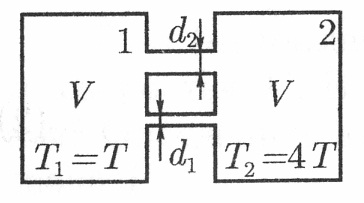
\includegraphics[width = 0.9 \textwidth]{0806KineticTheoryTwoVessels.jpg}
\end{minipage}
\begin{ans}
$\Delta M = 2M/15$
\end{ans}
\end{ex}

%Ижевск
\begin{ex}
\hspace{0pt} \\
\begin{minipage}{.65\textwidth}
Теплоизолированная полость небольшими малыми одинаковыми отверстиями соединена с двумя объемами, содержащими газообразный гелий. 
Давления в этих объемах поддерживаются одинаковыми и равными $P$, а температуры поддерживаются равными в одном из объемов $T$, в другом $2T$. 
Найдите установившиеся давление и температуру внутри полости.
\end{minipage}
\begin{minipage}{.35\textwidth}
\centering
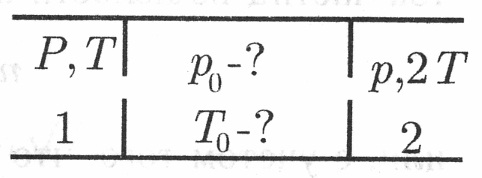
\includegraphics[width = 0.9 \textwidth]{0807KineticTheoryHelium.jpg}
\end{minipage}
\begin{ans}
$T_0 = \sqrt{2}T$, $p_0=p(1+\sqrt{2})2^{-5/4}$
\end{ans}
\end{ex}

%Ижевск
\begin{ex}
Плоская поверхность нагрета неравномерно, так что вдоль нее поддерживается градиент температуры $dT/dx$. 
В этих условиях газ, примыкающий к поверхности, приходит в движение вдоль поверхности. Это явление называют тепловым скольжением. 
Объясните его механизм и оцените скорость теплового скольжения. Необходимые параметры считать известными.
\begin{ans}
$u \approx \frac{\lambda}{2}\sqrt{\frac{k}{3mT}}\frac{dT}{dx}$
\end{ans}
\end{ex}

%Черепанов
\begin{ex}
(2008) Оценить по порядку величины установившуюся скорость, с которой будет двигаться в сильно разреженном воздухе плоский диск, одна из сторон которого нагрета до температуры $T_1$, а другая до температуры $T_2$, $T_1>T_2$. Температура воздуха равна $T$.
\begin{ans}
$u = \frac{\sqrt{T_2}-\sqrt{T_1}}{\sqrt{T_2}+\sqrt{T_1}+4\sqrt{T}} \sqrt{\frac{3RT}{\mu}}$
\end{ans}
\end{ex}

\begin{ex}
(2009) Каково должно быть максимальное значение температурного градиента $dT/dz$ атмосферного воздуха, 
чтобы он мог находиться в устойчивом механическом равновесии? Воздух считать двухатомным газом с относительной молекулярной массой $\mu$. 
Ускорение свободного падения $g$ не зависит от высоты над поверхностью земли.
\begin{ans}
$\mid \frac{dT}{dz} \mid < \frac{2\mu g}{7R}$
\end{ans}
\end{ex}